\documentclass[11pt]{amsart}
\usepackage{amsmath}
\usepackage{amssymb}
\usepackage{color}
\usepackage[T1]{fontenc}
\usepackage[utf8x]{inputenc}
\usepackage{xcolor}
\usepackage{tikz}

\begin{document}

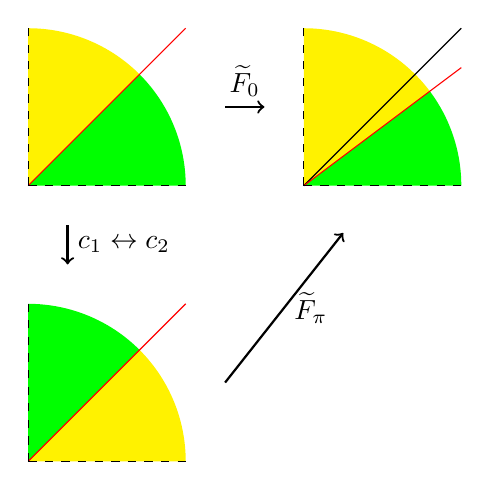
\begin{tikzpicture} 
    \fill[green] (0,0) -- (45:2) arc (45:0:2) -- (0,0);
    \fill[yellow] (0,0) -- (45:2) arc (45:90:2) -- cycle;
    \draw[red] (0,0) -- (2,2);
    \draw[dashed] (0,0) -- (2,0);
    \draw[dashed] (0,0) -- (0,2);
\begin{scope}[shift={(3.5,0)}]
\fill[green] (0,0) -- (37:2) arc (37:0:2) -- (0,0);
    \fill[yellow] (0,0) -- (37:2) arc (37:90:2) -- cycle;
    \draw (0,0) -- (2,2);
    \draw[red] (0,0) -- (2,3/2);
    \draw[dashed] (0,0) -- (2,0);
    \draw[dashed] (0,0) -- (0,2);
     \end{scope}
    \draw[->, thick] (2.5,1) -- (3,1) node[midway, above]{$\widetilde{F}_{0}$};
\begin{scope}[shift={(0,-3.5)}]    
\fill[yellow] (0,0) -- (45:2) arc (45:0:2) -- (0,0);
    \fill[green] (0,0) -- (45:2) arc (45:90:2) -- cycle;
    \draw[red] (0,0) -- (2,2);
    \draw[dashed] (0,0) -- (2,0);
    \draw[dashed] (0,0) -- (0,2);
\end{scope}
\draw[->, thick] (0.5,-0.5) -- (0.5,-1) node[midway, right]{$c_{1}\leftrightarrow c_{2}$};  
\draw[->, thick] (2.5,-2.5) -- (4,-0.6) node[midway, right]{$\widetilde{F}_{\pi}$};
\end{tikzpicture}

\end{document}